\chapter{Primera aproximación Greedy}
Para el desarrollo del proyecto, se han desarrollado dos algoritmos \textit{Greedy} para realizar tanto la asignación de las horas de teoría, como la asignación de horas y aulas de prácticas para cada grupo. Con esto en mente, podríamos ser capaces de inicializar una población inicial para un algoritmo genético, con el fin de optimizar más el horario generado, intentando que las soluciones generadas, saturen lo menos posible las aulas, no generen huecos a lo largo del turno de mañana o tarde, etc.

Aunque la filosofía de los algoritmos es bastante similar, hemos decidido dividir esta tarea en dos procesos, haciendo más fácil el desarrollo del código y la legibilidad de estos, además de facilizar la tarea al tener que ir examinando menos restricciones en cada paso del algoritmo. 

Para empezar, vamos a ver detalladamente el desarrollo del algoritmo voraz para las horas de teoría.

\section{Greedy para asignar horas de teoría}

Para que el algoritmo genético funcione bien, debemos asegurar que este tenga una buena diversidad en su población de soluciones. Como nuestra población inicial la generarán los algoritmos voraces, ambos tendrán un componente aleatorio para garantizar la diversidad en esta población. En \hyperref[greedyteoria]{Algoritmo \ref*{greedyteoria}}, podemos ver el pseudocódigo del algoritmo voraz para las horas de teoría.

% Para inicializar una población para el algoritmo genético, hemos desarrollado un algoritmo \textit{Greedy} aleatorio. El pseudocódigo se ve explicado en el \hyperref[greedyteoria]{Algoritmo \ref*{greedyteoria}} 

\begin{pseudocode}{GreedyTeoria}{ }
    \label{greedyteoria}
    \FOREACH g \in groups \DO
    \BEGIN
        d \GETS 0 \\
        subject\_list \GETS \CALL{shuffle}{\CALL{filter}{subjects, g}}\\
        \WHILE \sum subject\_list.th\_hours \neq 0 \DO
        \BEGIN
            \FOREACH s \in subject\_list \DO
            \BEGIN
                \IF s.th\_hours \neq 0 \DO
                \BEGIN
                    \IF g.turno = ``Morning'' \DO
                    \BEGIN
                        \FOR h \GETS 0 \TO number\_of\_hours / 2 \DO
                        \BEGIN
                            \IF \CALL{libre}{h} \DO
                            \BEGIN
                                tabla[d,h] \GETS (g, s, g.classroom)\\
                                s.th\_hours \GETS s.th\_hours - 1\\
                                d \GETS (d + 1) \bmod number\_of\_days\\
                                \BREAK
                            \END
                        \END
                    \END
                    \ELSE \DO
                    \BEGIN
                        \FOR h \GETS number\_of\_hours / 2 \TO number\_of\_hours \DO
                        \BEGIN
                            \IF \CALL{libre}{h} \DO
                            \BEGIN
                                tabla[d,h] \GETS (g, s, g.classroom)\\
                                s.th\_hours \GETS s.th\_hours - 1\\
                                d \GETS (d + 1) \bmod number\_of\_days\\
                                \BREAK
                            \END
                        \END
                    \END
                \END
            \END
        \END
    \END
\end{pseudocode}

Para empezar, tanto este algoritmo como el de prácticas, reciben cada uno como entrada el semestre para el que se va a calcular el horario. Esto se hace así, porque para cada semestre el horario es totalmente distinto, con lo que las restricciones que tiene cada uno son totalmente distintas, y no necesitan compartir nada. Con esto, se consigue simplificar el problema y la ejecución de este, aunque se tenga que ejecutar dos veces el algoritmo para poder obtener el horario de un año completo.

A continuación, el algoritmo lo que hace es para cada uno de los grupos, obtiene sus asignaturas. Esto se hace filtrando aquellas asignaturas que coincidadn en año, semestre y especialidad con el grupo que se está evaluando en cada iteración, y para asegurar una buena diversidad, a estas asignaturas se le aplica un ``shuffle'' o mezclado. Es decir, se obtiene una nueva permutación de asignaturas aleatoria.

Una vez hecho esto, el algoritmo entrará en un bucle del que no saldrá mientras que la suma total de horas de teoría que quedan por asignar al grupo no sea cero. En este bucle, irá recorriendo las asignaturas y las irá asignado una por día, en el primer hueco que encuentre en el horario, para el día correspondiente.

Esto se hace tanto para los grupos de mañana como para los grupos de tarde, y es capaz de generar un horario con las horas de teoría en tiempos muy pequeños.

Una de las ventajas que tiene este algoritmo frente al de prácticas, es que para cada grupo de teoría, se preasigna el aula en el que cursará las asignaturas a lo largo del año. Esto es así, porque reduce mucho la complejidad del problema, ya que si no fuera así, el espacio de búsqueda es tan grande, que la complejidad del problema crecería demasiado, haciendo extremadamente difícil la resolución de este problema.

Como aclaración, \texttt{number\_of\_hours} y \texttt{number\_of\_days} son atributos de la clase \texttt{Timetable}, y el atributo \texttt{th\_hours} de la clase \texttt{Subject} corresponde al número de horas teóricas de dicha asignatura. A continuación, podemos ver un ejemplo del funcionamiento del algoritmo.

%Para realizar el filtrado de asignaturas que pertenecen a cada grupo, filtramos aquellas asignaturas que coincidan tanto en año, como en semestre y especialidad con el grupo en cuestión. Este método pertenece a la clase \texttt{Timetable} y, por tanto, \texttt{tabla}, \texttt{number\_of\_hours} y \texttt{number\_of\_days} son atributos de dicha clase. El atributo \texttt{th\_hours} de la clase \texttt{Subject} corresponde al número de horas teóricas de dicha asignatura.

\subsection{Ejemplo de funcionamiento}
Supongamos que tenemos que hacer un horario para los grupos de segundo curso $A$ y $B$. Estos grupos, tienen como aula de teoría asignada la 0.1, y las asignaturas a cursar son:

\begin{enumerate}[$\bullet$]
    \item \textbf{AC} con dos horas de teoría.
    \item \textbf{ALG} con tres horas de teoría.
    \item \textbf{FBD} con una hora de teoría.
\end{enumerate}

Además de esto, tenemos que el horario escogido corresponde con una semana de tres días de longitud, y una jornada de cuatro horas, en las que hay que asignar estas asignaturas.

%Además, también suponemos que el número de días de en los que se quieren cuadrar estas asignaturas es de 3 y 4 horas.

% Vamos a hacer los pasos para cuadrar las asignaturas del grupo $A$:

A continuación, vamos a ver paso a paso cómo actúa el algoritmo para asignar las horas de teoría de forma correcta en nuestro horario.

\begin{minipage}{0.5\textwidth}    
\begin{tabular}{| c | c | c |}
\hline
 &  &  \\
 \hline
 &  &  \\
 \hline
 &  &  \\
 \hline
 &  &  \\
 \hline 
\end{tabular}
\end{minipage}
\begin{minipage}{0.5\textwidth}
\begin{tabular}{c | c}
Asignatura & Nº horas restantes \\
AC & 2 \\
ALG & 3 \\
FBD & 1
\end{tabular}
\end{minipage}

Seleccionamos la primera asignatura de nuestra lista filtrada y mezclada de asignaturas, \textbf{AC} y colocamos una de sus horas en el primer hueco disponible del horario. 

\begin{minipage}{0.5\textwidth}    
\begin{tabular}{| c | c | c |}
\hline
AC, A, 0.1 &  &  \\
 \hline
 &  &  \\
 \hline
 &  &  \\
 \hline
 &  &  \\
 \hline 
\end{tabular}
\end{minipage}
\begin{minipage}{0.5\textwidth}
\begin{tabular}{c | c}
Asignatura & Nº horas restantes \\
AC & 1 \\
ALG & 3 \\
FBD & 1
\end{tabular}
\end{minipage}

Ahora, hacemos lo mismo con \textbf{ALG} y \textbf{FBD}.

\begin{minipage}{0.5\textwidth}    
\begin{tabular}{| c | c | c |}
\hline
AC, A, 0.1 & ALG, A, 0.1  & FBD, A, 0.1 \\
 \hline
 &  &  \\
 \hline
 &  &  \\
 \hline
 &  &  \\
 \hline 
\end{tabular}
\end{minipage}
\begin{minipage}{0.5\textwidth}
\begin{tabular}{c | c}
Asignatura & Nº horas restantes \\
AC & 1 \\
ALG & 2 \\
FBD & 0
\end{tabular}
\end{minipage}

Como aún siguen quedando horas por asignar, damos otra vuelta más.

\begin{minipage}{0.5\textwidth}    
\begin{tabular}{| c | c | c |}
\hline
AC, A, 0.1 & ALG, A, 0.1  & FBD, A, 0.1 \\
 \hline
AC, A, 0.1 & ALG, A, 0.1 & ALG, A, 0.1  \\
 \hline
 &  &  \\
 \hline
 &  &  \\
 \hline 
\end{tabular}
\end{minipage}
\begin{minipage}{0.5\textwidth}
\begin{tabular}{c | c}
Asignatura & Nº horas restantes \\
AC & 0 \\
ALG & 0 \\
FBD & 0
\end{tabular}
\end{minipage}

Al no quedar más horas por asignar, pasaríamos a repetir estos mismos pasos con el grupo $B$.

\section{Greedy para inicializar horas de prácticas}
En el caso del Greedy para inicializar las horas de prácticas, hemos hecho un algoritmo parecido al algoritmo voraz de las horas de teoría. Su funcionamiento básico consiste en ir desplazando una ventana, cuyo tamaño será el número de subgrupos de prácticas, e ir asignando dicha ventana cada día de la semana.

\begin{pseudocode}{GreedyPracticas}{ }
    \label{greedypracticas}
    \FOREACH g \in groups \DO
    \BEGIN
        d \GETS 0 \\
        subject\_list \GETS \CALL{shuffle}{\CALL{filter}{subjects, g}}\\
        \WHILE \sum subject\_list.pr\_hours \neq 0 \DO
        \BEGIN
            \FOREACH v \in ventana\_subjects \DO
            \BEGIN
                \IF v.pr\_hours \neq 0 \DO
                \BEGIN
                    \IF g.turno = ``Morning'' \DO
                    \BEGIN
                        \FOR h \GETS 0 \TO number\_of\_hours / 2 \DO
                        \BEGIN
                            \IF \CALL{libre}{h} \DO
                            \BEGIN
                                tabla[d,h] \GETS (g, s)\\
                                s.th\_hours \GETS s.th\_hours - 1\\
                                d \GETS (d + 1) \bmod number\_of\_days\\
                                \BREAK
                            \END
                        \END
                    \END
                    \ELSE \DO
                    \BEGIN
                        \FOR h \GETS number\_of\_hours / 2 \TO number\_of\_hours \DO
                        \BEGIN
                            \IF \CALL{libre}{h} \DO
                            \BEGIN
                                tabla[d,h] \GETS (g, s, g.classroom)\\
                                s.th\_hours \GETS s.th\_hours - 1\\
                                d \GETS (d + 1) \bmod number\_of\_days\\
                                \BREAK
                            \END
                        \END
                    \END
                \END
            \END
        \END
    \END
\end{pseudocode}

Este algoritmo, al igual que antes, recibe como entrada el semestre para el cual se va a calcular el horario. Además de esto, ya no parte de un horario vacío, sino del horario que le ha dejado el algoritmo greedy para las horas de teoría, por lo que ya tiene una cierta ``estructura'' de partida.

Con esto, para cada uno de los grupos de prácticas, el algoritmo coge las asignaturas para ese grupo y para ese cuatrimestre, genera una permutación aleatoria de estas, y va asignando grupos de prácticas para cada día de la semana, siendo el siguiente día igual que el anterior, pero desplazada la ventana una posición hacia la derecha.

Una vez asignada una asignatura a una celda, se le resta una hora a las horas de prácticas a esta asignatura, para así, tener un control de qué asignaturas han sido asignadas y cuales no, y no asignar de nuevo aquellas que tengan ya cero horas de prácticas.

Este algoritmo funciona de forma parecida al algoritmo anterior, pero tiene la pecularidad de que, en función de las horas de prácticas que tengan las asignaturas, puede generar huecos en el horario o no. 

Estos huecos se generan cuando la cantidad de horas de prácticas de una asignatura es impar, como puede ser \textit{Cálculo} o \textit{Diseño y Desarrollo de Sistemas de Información}, que tienen una y tres horas de prácticas respectivamente. Esto provoca un efecto contrario al que queremos conseguir, minimizar los huecos en el horario, para que sea lo más compacto posible. 

Una forma de solucionar esto, fue que el algoritmo una vez asignadas todas las horas, en caso de quedar alguna hora sin asignar de alguna asignatura, asignara esa hora en alguno de los huecos que había en el horario, o bien, en una hora a parte. 

Esta solución es a su vez, un arma de doble filo debido a la componente aleatoria del algoritmo. Esto se debe a que es altamente probable que por la permutación que haya calculado el algoritmo, las horas de prácticas se vean seriamente afectadas, obteniendo un resultado en el que la primera hora de prácticas se asigna de forma correcta, y la segunda está desplazada una casilla hacia delante, haciendo el horario muy caótico e inútil.

Aun así, a continuación podemos ver un ejemplo de funcionamiento del algoritmo. 

\subsection{Ejemplo de funcionamiento}

A continuación podemos ver un ejemplo de uso del algoritmo para asignar las horas de prácticas a los distintos subgrupos de un grupo determinado. En este caso, es un grupo de segundo curso del Grado en Ingeniería Informática, más concretamente del segundo semestre.

En la \hyperref[pasig]{Tabla \ref*{pasig}}, podemos ver el conjunto de asignaturas del que se compone el semestre, junto con el número de horas de prácticas que corresponden a cada una de ellas.
%Supongamos que tenemos que asignar a un grupo con tres subgrupos de prácticas las siguientes asignaturas:
\begin{table}[H]
\center
\begin{tabular}{c | c  c  c  c  c}
\textbf{Nombre} & AC & FBD & ALG & IA & FIS \\
\hline
\textbf{Horas de prácticas}  & 2 & 3 & 1 & 2 & 2 \\
\end{tabular}
\caption{Asignaturas y horas correspondientes del segundo curso.}
\label{pasig}
\end{table}

En este caso, un grupo de segundo curso, tiene, como norma general, un número de alumnos lo suficientemente grande como para albergar tres subgrupos de prácticas, aunque esta información viene dada de antemano, antes de comenzar el algoritmo tanto de prácticas, para evitar cálculos innecesarios, que tienen una alta probabilidad de cambios y que pueden afectar al comportamiento del algoritmo.

Como esto es un caso de ejemplo, supondremos que este grupo de segundo tiene tres subgrupos de prácticas, por lo que, el tamaño de ventana a utilizar será de tres casillas. Además de esto, cada subgrupo de prácticas sabrá el número de horas restantes de prácticas que tiene por asignar, como se puede ver a continuación.

\begin{minipage}{0.5\textwidth}    
\begin{tabular}{| c | c | c | c | c |}
\hline
 &  &  &  & \\
 \hline
 &  &  &  & \\
 \hline
 &  &  &  & \\
 \hline
 &  &  &  & \\
 \hline 
\end{tabular}
\end{minipage}
\begin{minipage}{0.5\textwidth}
\begin{tabular}{c | c}
Asignatura & Nº horas restantes \\
AC & (2, 2, 2) \\
FBD & (3, 3, 3) \\
ALG & (1, 1, 1) \\
IA & (2, 2, 2) \\
FIS & (2, 2, 2)
\end{tabular}
\end{minipage}

En el primer paso, el algoritmo selecciona con la ventana las tres primeras asignauras de nuestra permutación de la \hyperref[pasig]{Tabla \ref*{pasig}}, (AC, FBD, ALG). Una vez seleccionados, el algoritmo empieza a recorrer el horario, y como el primer día que encuentra está libre, asigna las asignaturas de esta ventana a ese espacio libre.

%Seleccionamos las tres primeras asignaturas de la lista (AC, FBD, ALG), y las asignamos al primer día de la semana.

\begin{minipage}{0.5\textwidth}    
\begin{tabular}{| c | c | c | c | c |}
\hline
 (AC, A1), &  &  &  & \\
 (FBD, A2), &  &  &  & \\
 (ALG, A3) &  &  &  & \\
 \hline
 (AC, A1), &  &  &  & \\
 (FBD, A2), &  &  &  & \\
 (FBD, A3) &  &  &  & \\
 \hline
 &  &  &  & \\
 \hline
 &  &  &  & \\
 \hline 
\end{tabular}
\end{minipage}
\begin{minipage}{0.5\textwidth}
\begin{tabular}{c | c}
Asignatura & Nº horas restantes \\
AC & (0, 2, 2) \\
FBD & (3, 1, 2) \\
ALG & (1, 1, 0) \\
IA & (2, 2, 2) \\
FIS & (2, 2, 2)
\end{tabular}
\end{minipage}

Una vez asignada la ventana, es necesario reducir el número de horas que quedan por asignar a las asignaturas que han sido asignadas con la ventana. Esto se puede ver en la tabla anterior en el número de horas restantes para cada grupo.

Como siguiente paso, el algoritmo desplaza una posición a la derecha la ventana anterior, pasando de ser (AC, FBD, ALG) a ser (FBD, ALG, IA), y se vuelve a repetir la operación anterior.
%Movemos la ventana en una posición (FBD, ALG, IA) y volvemos a asignar las prácticas para el siguiente día de la semana:

\begin{minipage}{0.5\textwidth}    
\begin{tabular}{| c | c | c | c | c |}
\hline
 (AC, A1), & (FBD, A1), &  &  & \\
 (FBD, A2), & (ALG, A2) &  &  & \\
 (ALG, A3) &  (IA, A3) &  &  & \\
 \hline
 (AC, A1), & (FBD, A1) &  &  & \\
 (FBD, A2), & (FBD, A2) &  &  & \\
 (FBD, A3) & (IA, A3) &  &  & \\
 \hline
 &  &  &  & \\
 \hline
 &  &  &  & \\
 \hline 
\end{tabular}
\end{minipage}
\begin{minipage}{0.5\textwidth}
\begin{tabular}{c | c}
Asignatura & Nº horas restantes \\
AC & (0, 2, 2) \\
FBD & (1, 0, 2) \\
ALG & (1, 0, 0) \\
IA & (2, 2, 0) \\
FIS & (2, 2, 2)
\end{tabular}
\end{minipage}

Volvemos a mover la ventana una posición más (ALG, IA, FIS) y repetimos la operación del día anterior. En este caso, el grupo A1 tendrá un hueco en su segunda hora de prácticas, debido a que la asignatura ALG (Algorítmica) tiene una sola hora de prácticas, a diferencia del resto que tienen 2 y como excepción, FBD (Fundamentos de Bases de Datos) que tiene tres. Este hueco que queda ahí, se asignará más adelante, si es posible.

\begin{minipage}{0.7\textwidth}    
\begin{tabular}{| c | c | c | c | c |}
\hline
 (AC, A1), & (FBD, A1), & (ALG, A1) &  & \\
 (FBD, A2), & (ALG, A2) & (IA, A2) &  & \\
 (ALG, A3) &  (IA, A3) & (FIS, A3) &  & \\
 \hline
 (AC, A1), & (FBD, A1) & () &  & \\
 (FBD, A2), & (FBD, A2) & (IA, A2) &  & \\
 (FBD, A3) & (IA, A3) & (FIS, A3) &  & \\
 \hline
 &  &  &  & \\
 \hline
 &  &  &  & \\
 \hline 
\end{tabular}
\end{minipage}
\begin{minipage}{0.8\textwidth}
\begin{tabular}{c | c}
Asignatura & Nº horas restantes \\
AC & (0, 2, 2) \\
FBD & (1, 0, 2) \\
ALG & (0, 0, 0) \\
IA & (2, 0, 0) \\
FIS & (2, 2, 0)
\end{tabular}
\end{minipage}

Esta se repetirá hasta que se haya rellenado la semana completa, repitiendo el mismo proceso detallado anteriormente. 

\begin{minipage}{0.8\textwidth}    
\begin{tabular}{| c | c | c | c | c |}
\hline
 (AC, A1), & (FBD, A1), & (ALG, A1) & (IA, A1) & (FIS, A1) \\
 (FBD, A2), & (ALG, A2) & (IA, A2) & (FIS, A2) & (AC, A2) \\
 (ALG, A3) &  (IA, A3) & (FIS, A3) & (AC, A3) & (FBD, A3) \\
 \hline
 (AC, A1), & (FBD, A1) & () & (IA, A1) & (FIS, A1) \\
 (FBD, A2), & (FBD, A2) & (IA, A2) & (FIS, A2) & (AC, A2) \\
 (FBD, A3) & (IA, A3) & (FIS, A3) & (AC, A3) & (FBD, A3) \\
 \hline
 &  &  &  & \\
 \hline
 &  &  &  & \\
 \hline 
\end{tabular}
\end{minipage}
\begin{minipage}{1\textwidth}
\begin{tabular}{c | c}
Asignatura & Nº horas restantes \\
AC & (0, 0, 0) \\
FBD & (1, 0, 0) \\
ALG & (0, 0, 0) \\
IA & (0, 0, 0) \\
FIS & (0, 0, 0)
\end{tabular}
\end{minipage}

En este caso, se puede ver que la asignatura de FBD, tienen aún una hora por asignar, por lo que el algoritmo, tratará de asignarla en algún espacio en blanco que haya dejado el uso de la ventana, para reducir los ``huecos'' que puedan quedar en el horario. En este caso, se asignará en el hueco que dejó la asignatura de Algorítmica, optimizando el espacio. 

Pero en caso de que esta operación no sea posible, el algoritmo la asignará en un espacio donde no haya nada, como se puede ver en la \hyperref[horario]{Figura \ref*{horario}}.
% Como aún queda una hora por asignar, el algoritmo buscaría un hueco posible donde asignarla.

\begin{minipage}{0.8\textwidth}    
\begin{tabular}{| c | c | c | c | c |}
\hline
 (AC, A1), & (FBD, A1), & (ALG, A1) & (IA, A1) & (FIS, A1) \\
 (FBD, A2), & (ALG, A2) & (IA, A2) & (FIS, A2) & (AC, A2) \\
 (ALG, A3) &  (IA, A3) & (FIS, A3) & (AC, A3) & (FBD, A3) \\
 \hline
 (AC, A1), & (FBD, A1) & (FBD, A1) & (IA, A1) & (FIS, A1) \\
 (FBD, A2), & (FBD, A2) & (IA, A2) & (FIS, A2) & (AC, A2) \\
 (FBD, A3) & (IA, A3) & (FIS, A3) & (AC, A3) & (FBD, A3) \\
 \hline
 &  &  &  & \\
 \hline
 &  &  &  & \\
 \hline 
\end{tabular}
\end{minipage}
\begin{minipage}{1\textwidth}
\begin{tabular}{c | c}
Asignatura & Nº horas restantes \\
AC & (0, 0, 0) \\
FBD & (0, 0, 0) \\
ALG & (0, 0, 0) \\
IA & (0, 0, 0) \\
FIS & (0, 0, 0)
\end{tabular}
\end{minipage}

\begin{figure}[H]
    \centering
    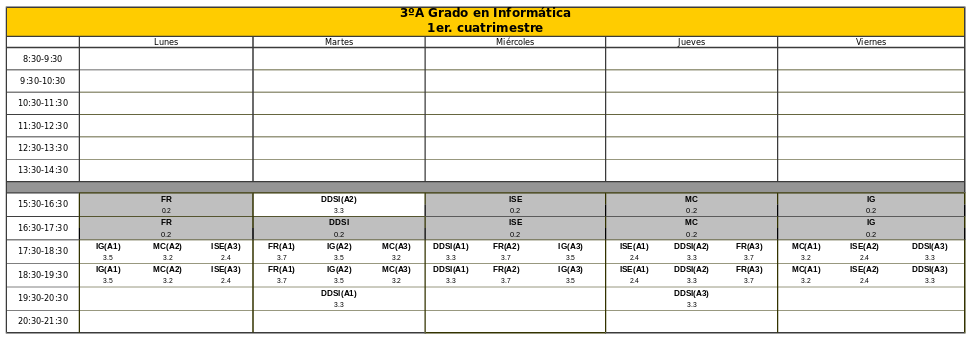
\includegraphics[width=\textwidth]{img/horario}
    \caption{Caso en el que una hora de prácticas no es posible asignarla en ningún espacio.}
    \label{horario}
\end{figure}

Con esto, el algoritmo de asignación de horas de prácticas finaliza, quedando todas las asignaturas asignadas a días, para todos los grupos de prácticas.

\subsection{Asignación de aulas de prácticas}
Consideramos que la mejor asignación es la que tiene en cuenta el material que necesita cada asignatura para llevar a cabo sus prácticas y el material del que dispone cada aula. Por ejemplo, para la asignatura \textit{Fundamentos de Redes} se necesita usar un aula con una instalación de red especial, por lo que no puede ser asignada en un aula que no disponga de dicha instalación. 

Por tanto, para calcular qué aula es la óptima para cada asignatura, debemos saber qué materiales necesita cada asignatura y qué materiales dispone cada aula. Para saber los materiales de los que dispone cada aula, hemos consultado la página web de la escuela: \url{http://etsiit.ugr.es/pages/instalaciones_servicios/aulas_etsiit2017/!}.

Nuestro algoritmo elige las asignaturas más restrictivas (con una lista de materiales más larga) y les asigna las aulas óptimas. Termina con las asignaturas que \textit{podrían} impartirse en ``cualquier'' aula.

\section{Problemas con esta primera aproximación}
A la hora de implementar esta versión nos hemos encontrado con varios problemas:

\begin{enumerate}[---]
    \item El principal problema de esta forma de asignar los horarios, es que las horas de prácticas se asignaban en la misma franja horaria, es decir, todas las horas de teoría se situaban de 8:30 a 10:30 en el caso del turno de mañana, o de 15:30 a 17:30 en el caso del horario de tarde.

    Esto supone que, las clases de teoría estén muy saturadas, pudiendo darse el caso de que a la misma hora, haya dos grupos de teoría que tengan que dar la clase en el mismo aula, lo que produce una saturación en las aulas de teoría.

    Este problema se agrava mucho más a la hora de asignar las aulas de prácticas, debido al espacio limitado y que todos los grupos de cada turno, comenzaban las prácticas a la misma hora, produciéndose tal saturación, que a la hora de asignar el aula, no acababa en la gran mayoría de los casos, siendo extremadamente difícil asignar aulas a los distintos subgrupos de prácticas de la escuela, y además, realizando una ejecución sólo para el Grado en Ingeniería Informática.

    Un intento de solución que se hizo, que mejoró algo este problema, fue asignar cuándo comenzaban las clases de teoría para cada día lanzando un aleatorio, para elegir si las clases de teoría comenzarían de 8:30 a 10:30, o bien de 10:30 a 12:30, siendo igual para el turno de tarde.

    En este caso se dio la misma probabilidad a ambas franjas horarias, para no favorecer ninguna y permitir que las clases de prácticas estuvieran más distribuidas y disminuir la saturación de aulas que generaba este algoritmo.

    Esta nueva versión, mejoró algo la situación para los cursos de primero y segundo, teniendo ya algunos problemas para las aulas de tercero, y volviendo a tener los mismos problemas de saturiación para los cursos de cuarto, siendo difícil realizar una asignación de aulas correcta.

    Esto se soluciona haciendo primero una estructura de horarios, en la que hiremos marcando para cada una de las diferentes horas del horario, si corresponde a una hora de teoría de prácticas o de teoría, con el fin de que realizando esta estructura, el algoritmo sea capaz de no sobresaturar las horas de prácticas o teoría. Esto se hace antes de asignar asignaturas tanto de teoría o de prácticas, procurando que si a un grupo a cierta hora le ha asignado una hora de teoría, el siguiente grupo, a esa hora, tendrá una hora de prácticas. Más adelante se podrá encontrar esto con más detalle.

    \item No es posible realizar una asignación óptima de las aulas de prácticas. Esto se debe a que para hacer una asignación óptima de las aulas, es necesario conocer de antemano los materiales de los que dispone cada aula. En el caso de la Escuela Técnica de Ingeniería Informática, es posible obtener la información exacta de cada aula en la página web de la escuela, como hemos mencionado anteriormente.

    El problema está en que cada año este material puede cambiar, al igual que puede cambiar el material que necesita cada asignatura, o cada profesor. Esto hace, que para cada asignatura, cada profesor pueda tener unos requisitos de materiales distintos al resto de profesores para esa asignatura. Por tanto, esto dificulta muchísimo la asignación óptima de aulas de prácticas.

    En nuestra primera aproximación, hicimos una ejecución para crear los horarios sólo del Grado en Ingeniería Informática, donde nosotros asignamos a mano los materiales que necesitaba cada asignatura, muchas por conocimiento propio tras cursar las asignaturas y otras por consultas a compañeros de otras especialidades y de otros años. El resultado tenía cierta aproximación a la asignación de aulas actual, pero no tenía tanta calidad como para presentarlo como resultado final, además de que era para un solo grado. 

    Esto, a la hora de meter más grados, y meter un conocimiento al problema que no era nuestro, comenzó a dar serios problemas para asignar las aulas, ya que había restricciones tan fuertes de materiales, que en algunos casos, ya no era posible asignar las aulas de prácticas, produciendo ciclos y que el programa no acabase en la mayoría de casos, y en los que acababa, el horario resultante, en términos de calidad por horario comprimido y sin huecos en medio de la jornadad, muy malo. 

    Es por esto por lo que decidimos cambiar la forma en la que asignamos las aulas de prácticas, de modo que ya no fuera necesario conocer de forma previa los materiales de las aulas, materiales de cada asignatura, etc. Más adelante, se explicará la siguiente versión del algoritmo para realizar esta tarea, junto con sus ventajas y desventajas.

\end{enumerate}
